\documentclass[11pt,a4paper]{article}
\usepackage[T1]{fontenc}
\usepackage[utf8]{inputenc}
\usepackage{lmodern,microtype}
\usepackage{amsmath,amssymb,amsthm,mathtools,bm}
\usepackage{booktabs,array,tabularx,longtable}
\usepackage{graphicx,float,caption}
\usepackage{xcolor}
\usepackage[margin=22mm]{geometry}
\usepackage{enumitem}
\usepackage{fancyhdr}
\usepackage[hidelinks]{hyperref}
\hypersetup{
  pdftitle={FIN Programs P517-P526: Fourth-Jet Obstruction, Stability Boundary, and Frequency Torus},
  pdfauthor={Krzysztof Żuchowski},
  pdfsubject={Information-functional source obstruction, interval orbital stability, memory dynamics, frequency independence, context bounds, robust observability},
  pdfkeywords={FIN, DNLS, information functional, Krawczyk, orbital stability, memory kernel, Lindemann-Weierstrass, spectral clock, identifiability}
}
\setlength{\parindent}{0pt}
\setlength{\parskip}{0.55em}
\setlength{\headheight}{14pt}
\setlist[itemize]{leftmargin=1.6em,itemsep=0.2em,topsep=0.2em}
\pagestyle{fancy}
\fancyhf{}
\lhead{FIN Programs P517--P526}
\rhead{Release 10.52}
\cfoot{\thepage}
\newtheorem{theorem}{Theorem}[section]
\newtheorem{proposition}[theorem]{Proposition}
\newcommand{\proven}{\textcolor{green!50!black}{\textbf{[PROVEN]}}}
\newcommand{\strong}{\textcolor{blue!70!black}{\textbf{[STRONG EVIDENCE]}}}
\newcommand{\conditional}{\textcolor{black!60}{\textbf{[CONDITIONAL]}}}
\newcommand{\moderate}{\textcolor{orange!85!black}{\textbf{[MODERATE EVIDENCE]}}}
\newcommand{\refuted}{\textcolor{red!75!black}{\textbf{[REFUTED CANDIDATE]}}}
\newcommand{\claimbox}[1]{\begin{center}\fcolorbox{blue!60!black}{blue!4}{\parbox{0.91\textwidth}{#1}}\end{center}}

\begin{document}

\pagenumbering{gobble}
\begin{titlepage}
\centering
\vspace*{2.0cm}
{\LARGE\bfseries FIN Programs P517--P526\par}
\vspace{0.7cm}
{\Large Fourth-Jet Obstruction, Stability Boundary,\par and the Six-Frequency Torus\par}
\vspace{0.5cm}
{\large Exact replay, memory falsification, context certification, and robust observability\par}
\vspace{1.6cm}
{\Large Krzysztof Żuchowski\par}
\vspace{0.3cm}
{\large Independent Researcher --- Fractal Information Theory Project\par}
{\large ORCID: 0009-0002-0909-3613\par}
\vspace{1.4cm}
{\large FIN Release 10.52 --- Version 1.0.0\par}
{\large 10 August 2026\par}
\vfill
\begin{minipage}{0.82\textwidth}
\textbf{Scope.} This report executes the ten bounded local studies P517--P526 recommended by Release 10.51. It tests the missing nonlinear source, upgrades the finite DNLS stability ledger, and distinguishes stationary memory persistence from stability of a temporal realization.\par
\textbf{Evidence boundary.} Exact finite algebra, outward interval arithmetic, exact replay of exported ledgers, finite numerical dynamics and synthetic operational models are admitted. No laboratory record, external audit, dimensional calibration or particle identification is asserted.\par
\textbf{Runtime.} The deterministic batch ran locally in approximately 24.2 seconds. Twelve regression and certificate tests passed.\par
\textbf{Repository.} \url{https://github.com/hyconiek/Fractal-Nadsoliton-Theory}\par
\textbf{License.} CC BY 4.0.
\end{minipage}
\end{titlepage}
\pagenumbering{arabic}

\begin{abstract}
Ten follow-up studies sharpen both the positive and negative mathematical content of the FIN strict-operator programme. P517 proves that attaching the words entropy, Fisher information or compression to an action does not select the focusing quartic jet required by the localized DNLS state. In the natural local invariant class, an arbitrary coefficient multiplying $\sum_x|\psi_x|^4$ remains invisible to the quadratic strict core. Positive convex relative information selects the opposite, defocusing sign; focusing requires an objective reversal or a separate nonlinear response law.

P518 exports and exactly replays all 801 outward Krawczyk acceptance inequalities underlying the P508 branch certificate. P519 substantially strengthens the dynamical result: 208 parametric state charts and 207 nested interface certificates cover $0.68\leq\omega\leq1.20$. Weyl margins prove the required finite $L_-/L_+$ inertia throughout. On $[0.99,1.01]$, $dP/d\omega\in[0.54242,0.69264]$. The unique VK sign transition in $[0.70,0.75]$ lies in
\[
 [0.722143668857225,\ 0.722143708857225],
\]
and the certified curvature lower bound there is $3.56036$.

P520 identifies the bond-to-uniform transition as the mode-one uniform bifurcation $\omega=\lambda_1/2=0.3770605771\ldots$. No separate fold is resolved away from that transition. Fifteen phase-kick trials yield no state that is simultaneously translating and localized; the largest apparent displacement is accompanied by delocalization. P521 then falsifies a tempting inference from stationary memory robustness: in an explicit causal three-pole hidden-relaxation completion, a positive growth rate already occurs at memory loading $0.01$. Stationary survival therefore does not imply temporal stability.

P522 proves an exact arithmetic theorem. The six distinct positive strict frequencies are linearly independent over the algebraic numbers. The exact distance-to-mode determinant is $-3456\sqrt3$. They generate a six-dimensional quasiperiodic frequency torus, but the rescaling $(A,t)\mapsto(cA,t/c)$ proves that no absolute clock unit follows. P523 transfers a fractional $n^{-0.8}$ context certificate to $C_{384}$ with maximum normalized bound $0.06708$, conditional only on a stated FFT rounding model. P524 provides an exact standard-library replay of the 573-box PSD ledger. P525 constructs a seven-variable detector-error polytope, while P526 proves again---now with frozen hold-out data---that finite model ranking cannot identify an unrestricted causal bridge law.

The principal conclusion is precise: the finite strict operator now supports a certified localized branch and a certified stability sector after a focusing fourth-order jet is supplied. Neither information terminology nor the spectrum itself supplies that jet, its scale, or dimensional physics.
\end{abstract}

\textbf{Status vocabulary.} \proven{} denotes an analytic theorem or exact/outward finite certificate in its declared model; \strong{} denotes robust finite numerical evidence; \conditional{} marks an added law, rounding model, environment or operational budget; \moderate{} denotes bounded incomplete evidence; \refuted{} denotes failure of a precisely stated candidate.

\tableofcontents
\newpage

\section{Executive results}

\claimbox{\textbf{Central result.} The mathematical localization and its favourable finite stability sector are now certificate-level results inside the supplied focusing DNLS. The attempt to derive that focusing jet from generic information functionals fails: its sign, strength, reference measure and dimensional conversion remain independent typed data.}

\begin{longtable}{@{}p{0.07\textwidth}p{0.23\textwidth}p{0.40\textwidth}p{0.22\textwidth}@{}}
\caption{Programs, generated objects and terminal verdicts.}\\
\toprule
ID & New object & Main result & Status\\
\midrule
\endfirsthead
\toprule
ID & New object & Main result & Status\\
\midrule
\endhead
P517 & O221 information fourth-jet obstruction & Standard information functionals do not uniquely select focusing sign or magnitude. & \proven\\
P518 & O222 exact O212 replay ledger & All 401 charts and 400 interface inclusions replay with exact rational inequalities. & \proven\\
P519 & O223 interval GSS/VK tube & A connected certified branch and inertia ledger cover $[0.68,1.20]$; the VK transition is isolated. & \proven{} / \conditional\\
P520 & O224 bond-bifurcation/kick ledger & Bond state joins the uniform mode-one bifurcation; no localized translating kick survives the scan. & \strong{} / \refuted\\
P521 & O225 temporal memory realization & The declared hidden-relaxation completion develops a positive growth exponent. & \strong{} / \conditional\\
P522 & O226 six-frequency certificate & Six positive strict frequencies are algebraically linearly independent; absolute scale remains impossible. & \proven\\
P523 & O227 fractional context certificate & The $C_{384}$ normalized limit error is bounded by $0.06708$ under the declared rounding model. & \proven{} / \conditional\\
P524 & O228 portable PSD ledger & Exact standard-library replay verifies 573 boxes and one unresolved connected bracket. & \proven\\
P525 & O229 detector-error polytope & Seven explicit error coordinates define a nonempty conservative separation region. & \conditional\\
P526 & O230 frozen-holdout law audit & Candidate ranking changes with regularization; unrestricted finite-record identification is impossible. & \proven{} / \conditional\\
\bottomrule
\end{longtable}

\section{Shared model and noninheritance rule}

The finite strict working generator is
\[
 W_{xy}=\frac{\cos(0.18575d(x,y)+0.16250)}{1+d(x,y)^{9/5}},
 \qquad A=\operatorname{diag}(W\mathbf1)-W\succeq0
\]
on $\mathbb Z/12\mathbb Z$. The nonlinear branch is defined only after adding
\begin{equation}
 i\dot\psi=A\psi-|\psi|^2\psi,
 \qquad Au+\omega u-u^{\circ3}=0.                 \label{eq:dnls52}
\end{equation}
The focusing cubic sign in \eqref{eq:dnls52} is not silently attributed to the strict kernel. Nor is the strict kernel identified with the legacy ontological kernel. No legacy electromagnetic, hierarchy, Planck-scale, matter or gravity role is transferred in this report.

\section{P517 --- information does not yet source the focusing jet}

Put $\rho_x=q+|\psi_x|^2$ around a positive reference $q$. Relative entropy has
\[
 D(\rho\Vert q)=\sum_x\left(\rho_x\log\frac{\rho_x}{q}-\rho_x+q\right)
 =\frac{1}{2q}\sum_x|\psi_x|^4+O(|\psi|^6).
\]
For $q=1/12$ the quartic coefficient is $+6$, hence positive minimization produces the defocusing sign. The functional $-D$ has coefficient $-6$ and produces focusing, but the sign reversal is an additional choice and abandons convex codelength minimization. Pearson information has the same positive curvature. Normalized Shannon entropy loses radial scale; Fisher information supplies gradient structure rather than an onsite quartic coefficient.

\begin{theorem}[Information-label insufficiency]
Within local $U(1)$- and permutation-invariant amplitude actions compatible with the supplied quadratic core, the coefficient $c$ in
\[
 E_c(\psi)=\frac12\langle\psi,A\psi\rangle+c\sum_x|\psi_x|^4+O(|\psi|^6)
\]
is not determined by the value, gradient or Hessian at the vacuum. Entropy, Fisher and compression labels do not remove this freedom without a reference measure, an extremum direction and a coupling normalization.
\end{theorem}

\textit{Consequence.} A genuine FIN source theorem must supply at least those three data. If the result is to be physical, a dimensional conversion is a fourth independent obligation.

\begin{figure}[H]
\centering
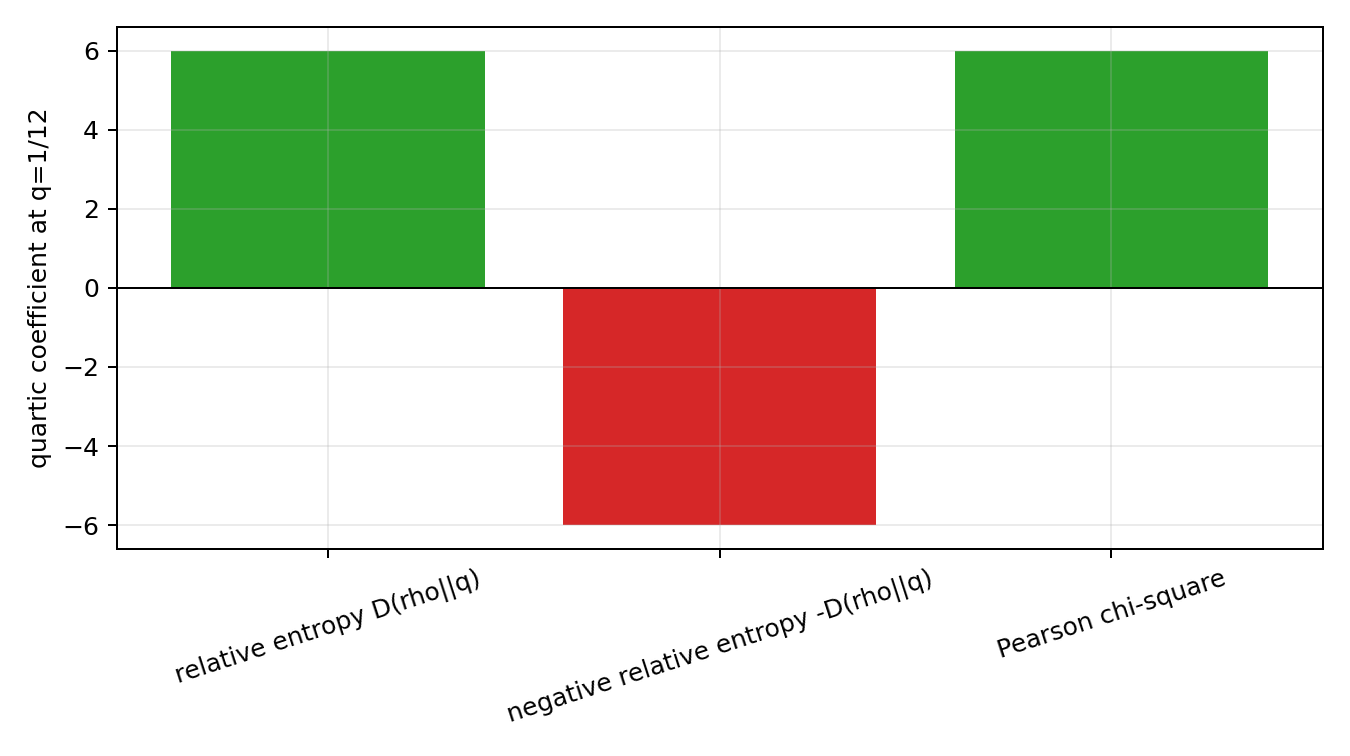
\includegraphics[width=0.78\textwidth]{FIN_Programs_517_526_Figures/p517_information_quartic_sign.png}
\caption{Opposite fourth-order jets arise from equally recognizable information objectives. The labels alone do not select focusing.}
\end{figure}

\section{P518 --- exact replay of the complete branch certificate}

The O212 generator was rerun using one common rational boundary partition. It exports 401 parameter-chart inequalities and 400 shared-parameter bridge inequalities. Every hexadecimal binary64 endpoint is an exact dyadic rational. A standard-library checker converts them to \texttt{Fraction} and verifies:
\begin{itemize}
\item every inclusion margin is positive;
\item every Krawczyk defect upper bound is below one;
\item every bridge root box is nested in both adjacent state boxes;
\item the parameter intervals form a complete partition of $[0,1]$.
\end{itemize}
The minimum exported inclusion margin is $1.996\times10^{-11}$, the maximum defect is $0.00627510$, and the minimum nesting margin is $4.704\times10^{-6}$.

\textbf{Trust boundary.} This is an exact replay of the outward acceptance ledger, not a second implementation of transcendental interval generation. The latter remains upstream in the mpmath-based generator.

\section{P519 --- a connected interval stability tube}

For a real stationary state define
\[
 L_-=A+\omega I-\operatorname{diag}(u^2),\qquad
 L_+=A+\omega I-3\operatorname{diag}(u^2).
\]
The state equation gives $L_-u=0$. A favourable finite GSS/VK ledger requires a positive second eigenvalue of $L_-$, exactly one negative direction of $L_+$, and the appropriate sign of
\[
 \frac{dP}{d\omega}=-2u^TL_+^{-1}u.
\]

P519 constructs 208 outward state charts over $[0.68,1.20]$ and 207 point root boxes nested at their interfaces. Thus the certified roots belong to one connected branch. Interval Weyl bounds certify the inertia in every chart. Verified linear solves enclose $u'=-L_+^{-1}u$ and $u''$.

On $0.99\leq\omega\leq1.01$:
\[
 \lambda_2(L_-)\ge1.20135,\quad
 \lambda_1(L_+)\le-4.31408,\quad
 \lambda_2(L_+)\ge0.968515,
\]
and
\[
 0.5424198\le \frac{dP}{d\omega}\le0.6926365.
\]
The slope changes sign in
\[
 \omega_*\in[0.722143668857225,\ 0.722143708857225].
\]
On $[0.70,0.75]$ the lower bound for $d^2P/d\omega^2$ is $3.56036$, proving uniqueness of this sign transition in that interval.

\begin{theorem}[Conditional finite stability sector]
For the supplied focusing finite DNLS and declared strict decimal operator, the site-centred branch has the certified GSS/VK inertia on $[0.68,1.20]$. Its VK slope is positive above the unique enclosed transition and negative below it. In particular the neighbourhood $[0.99,1.01]$ satisfies the favourable finite orbital-stability sign conditions.
\end{theorem}

The theorem is about the added DNLS model; it does not source that law or promote it to laboratory physics.

\begin{figure}[H]
\centering
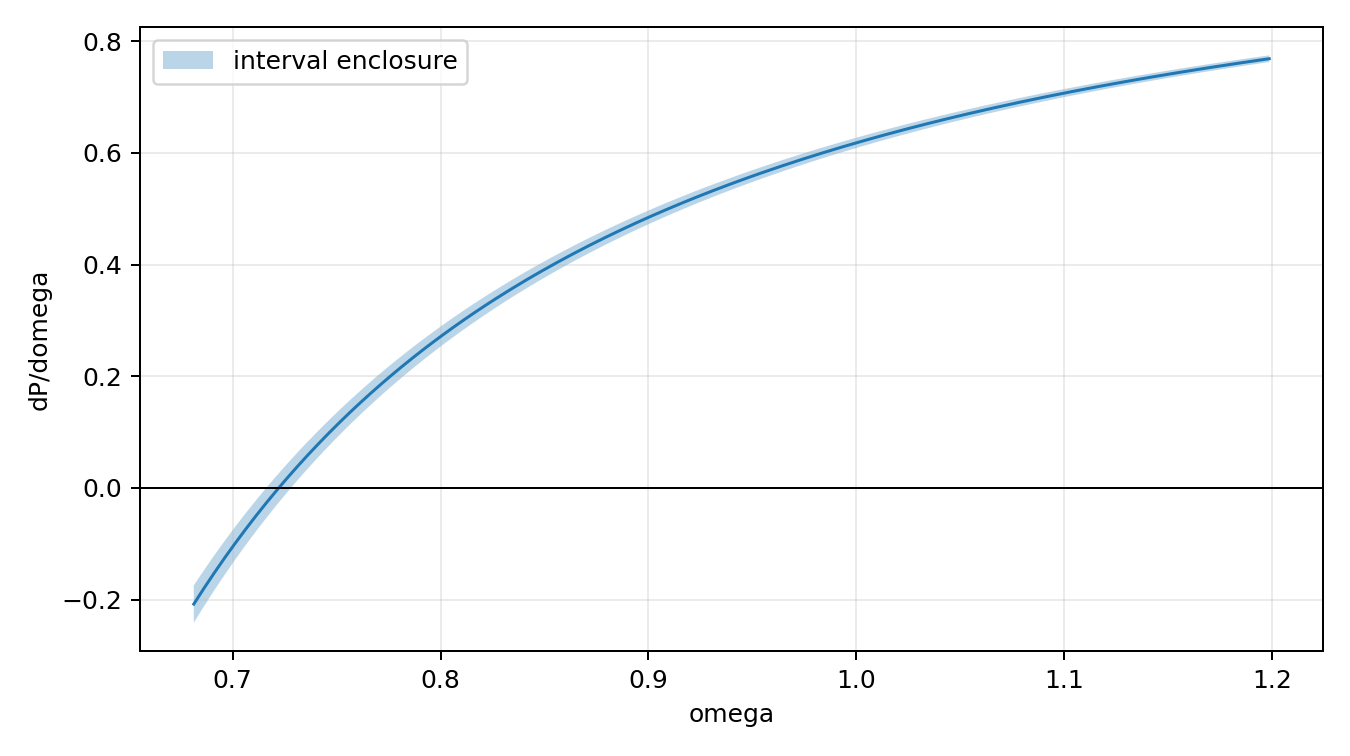
\includegraphics[width=0.78\textwidth]{FIN_Programs_517_526_Figures/p519_interval_vk_tube.png}
\caption{Outward enclosure of $dP/d\omega$ across the certified frequency tube.}
\end{figure}

\section{P520 --- bond bifurcation and the failed mobility candidate}

The uniform stationary state $u_x=\sqrt\omega$ loses invertibility when
\[
 L_+^{\rm unif}=A-2\omega I
\]
has a zero eigenvalue, hence at $\omega_m=\lambda_m(A)/2$. The descending bond-centred branch becomes nearly uniform between $0.378$ and $0.376$. Its last nonuniform deviation is dominated by mode one, and the corresponding exact finite spectral prediction is
\[
 \omega_1=\frac{\lambda_1(A)}2=0.3770605771035399.
\]
No additional small-singular-value fold is found away from this transition in the declared scan.

Fifteen phase-kicked site states were then evolved to time 60 with power and energy drift below $10^{-9}$. No trial met all three preregistered conditions: displacement of at least one site, minimum IPR at least $0.25$, and directional monotonicity at least $0.8$. The largest apparent displacement occurred for kick $1.3$, but its minimum IPR was only $0.10057$; it transported a delocalized density pattern, not a coherent breather.

\textbf{Verdict.} The scanned phase kick does not repair the missing equal-power PN comparison. This falsifies one bounded mobility proposal, not every possible travelling solution.

\begin{figure}[H]
\centering
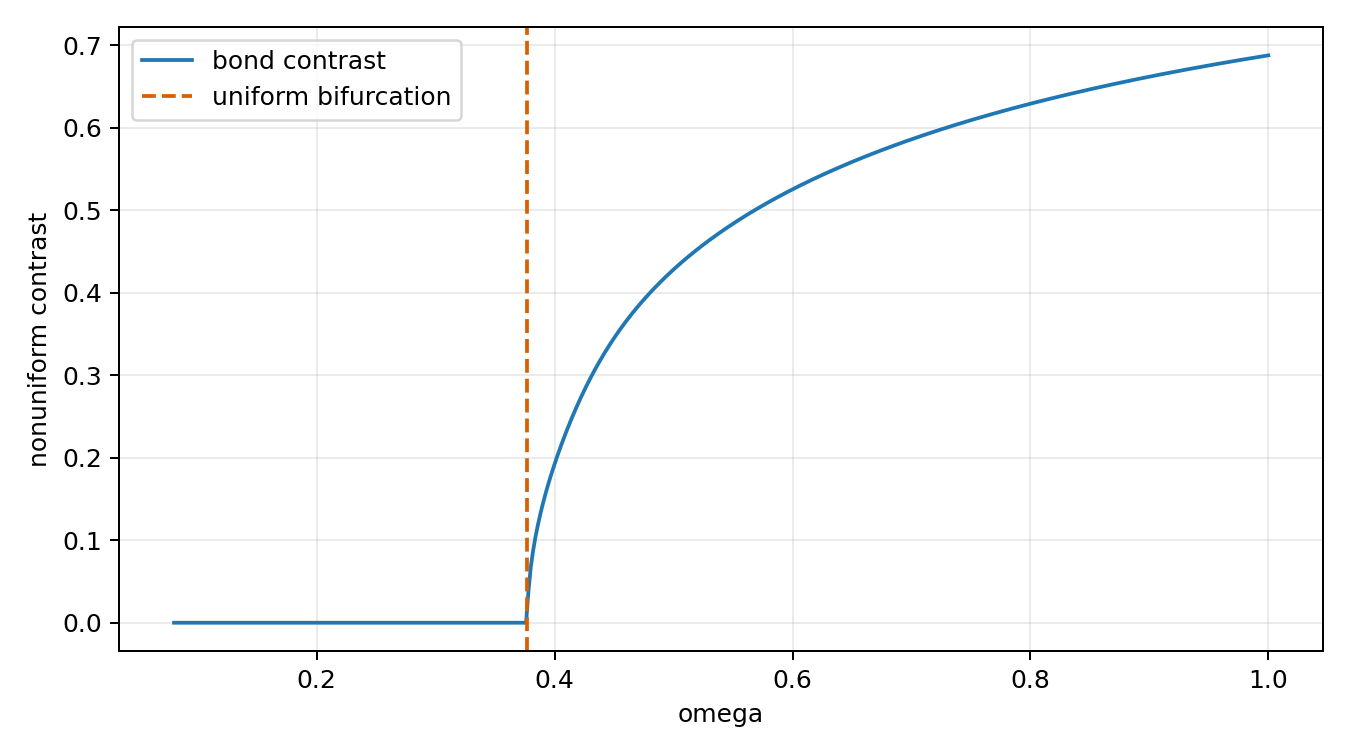
\includegraphics[width=0.78\textwidth]{FIN_Programs_517_526_Figures/p520_bond_bifurcation.png}
\caption{Bond contrast collapses at the independently predicted mode-one uniform bifurcation.}
\end{figure}

\section{P521 --- stationary memory persistence is not temporal stability}

The three-pole Stieltjes response is realized by complex hidden variables:
\begin{align*}
 i\dot\psi&=A\psi+\omega\psi-|\psi|^2\psi
 +\varepsilon\left(\sigma(0)\psi-\sum_jr_jy_j\right),\\
 \dot y_j&=\psi-(A+c_jI)y_j,\qquad c_j,r_j>0.
\end{align*}
At equilibrium $y_j=(A+c_jI)^{-1}u$, reproducing the stationary memory operator of P511. The real linearization has dimension $96$. Its complete floating spectrum was evaluated at 101 loadings.

At $\varepsilon=0.01$ a nonneutral eigenvalue already has real part $0.0111125$; the maximum spectral abscissa reaches $0.672779$ by full loading. The phase-neutral eigenvalue remains at residual scale $1.83\times10^{-13}$.

\claimbox{\textbf{Falsification.} The statement ``the localized stationary solution survives memory loading'' does not imply ``a causal temporal realization of that memory is stable''. The declared hidden-relaxation realization is a concrete counterexample at strong numerical-evidence level. It does not prove that every passive or Hamiltonian memory realization is unstable.}

\begin{figure}[H]
\centering
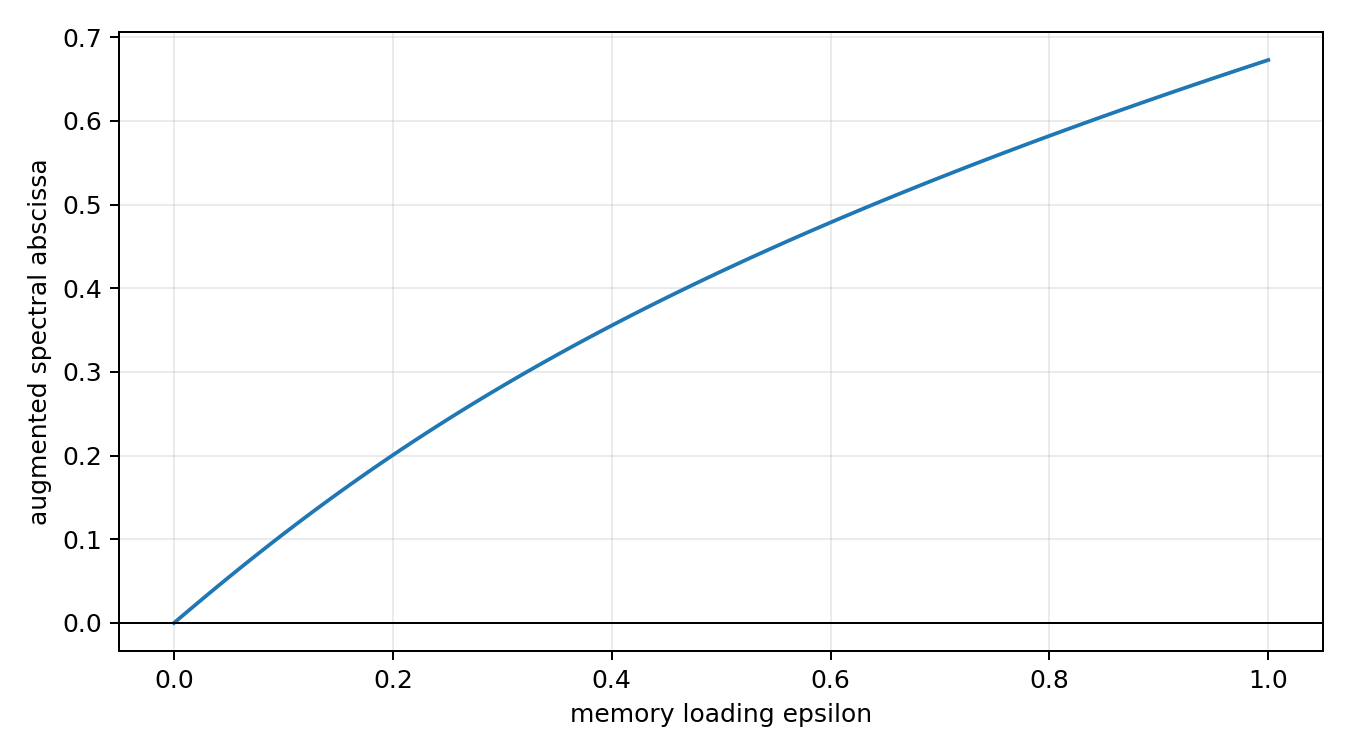
\includegraphics[width=0.78\textwidth]{FIN_Programs_517_526_Figures/p521_memory_spectral_abscissa.png}
\caption{The augmented spectral abscissa becomes positive immediately under the declared temporal memory loading.}
\end{figure}

\section{P522 --- the maximal six-frequency torus and scale no-go}

Let $z=e^{i/4000}$. Each distance weight is a Laurent polynomial in $z$ with algebraic coefficients and a distance-specific highest exponent. The six distinct positive Laplacian frequencies satisfy
\[
 (\lambda_1,\ldots,\lambda_6)^T=C(w_1,\ldots,w_6)^T,
\]
where
\[
 C_{md}=\begin{cases}
 2\bigl(1-\cos(2\pi md/12)\bigr),&d<6,\\
 1-(-1)^m,&d=6.
 \end{cases}
\]
Exact symbolic calculation gives
\[
 \det C=-3456\sqrt3\ne0.
\]

\begin{theorem}[Maximal algebraic linear independence]
The six distinct positive strict frequencies $\lambda_1,\ldots,\lambda_6$ are linearly independent over the algebraic numbers and therefore rationally independent. Six is maximal because the remaining nonzero modes are the degeneracies $\lambda_{12-m}=\lambda_m$.
\end{theorem}

\textit{Proof sketch.} An algebraic linear relation among the frequencies gives one among the six Laurent-polynomial weights because $C$ is invertible. The unique highest powers then force every coefficient to vanish, since $z$ is transcendental by Lindemann--Weierstrass.

This supplies a genuine six-frequency quasiperiodic clock torus. It still does not supply a physical clock. For every $c>0$,
\[
 e^{-it(cA)}=e^{-i(ct)A};
\]
equivalently $(A,t)\mapsto(cA,t/c)$ preserves all dimensionless orbits and spectral ratios. Absolute duration and energy are unidentifiable from the dimensionless operator alone.

\section{P523 --- a useful C384 context bound}

The attenuation tail has Hölder exponent $\eta-1=0.8$. P513's direct constants could not certify a positive normalized denominator at $C_{384}$. P523 instead uses a multilevel route:
\[
 \|F_{384}-F_\infty\|
 \le \|F_{384}-F_{262144}\|
 +\|F_{262144}-F_\infty\|.
\]
The first term is a finite deterministic comparison. The second is paid by the analytic Wiener/resolvent $n^{-0.8}$ envelope. Including a conservative $2\times10^{-9}$ IEEE-FFT rounding allowance gives a maximum normalized bound
\[
 \max_u|F_{384}(u)-F_\infty(u)|\le0.0670791.
\]
This is far larger than the observed $C_{384}$ discrepancy but is finally informative at the requested context size. The result remains conditional on the explicit FFT rounding model; an interval radix-two transform would remove that dependency.

\begin{figure}[H]
\centering
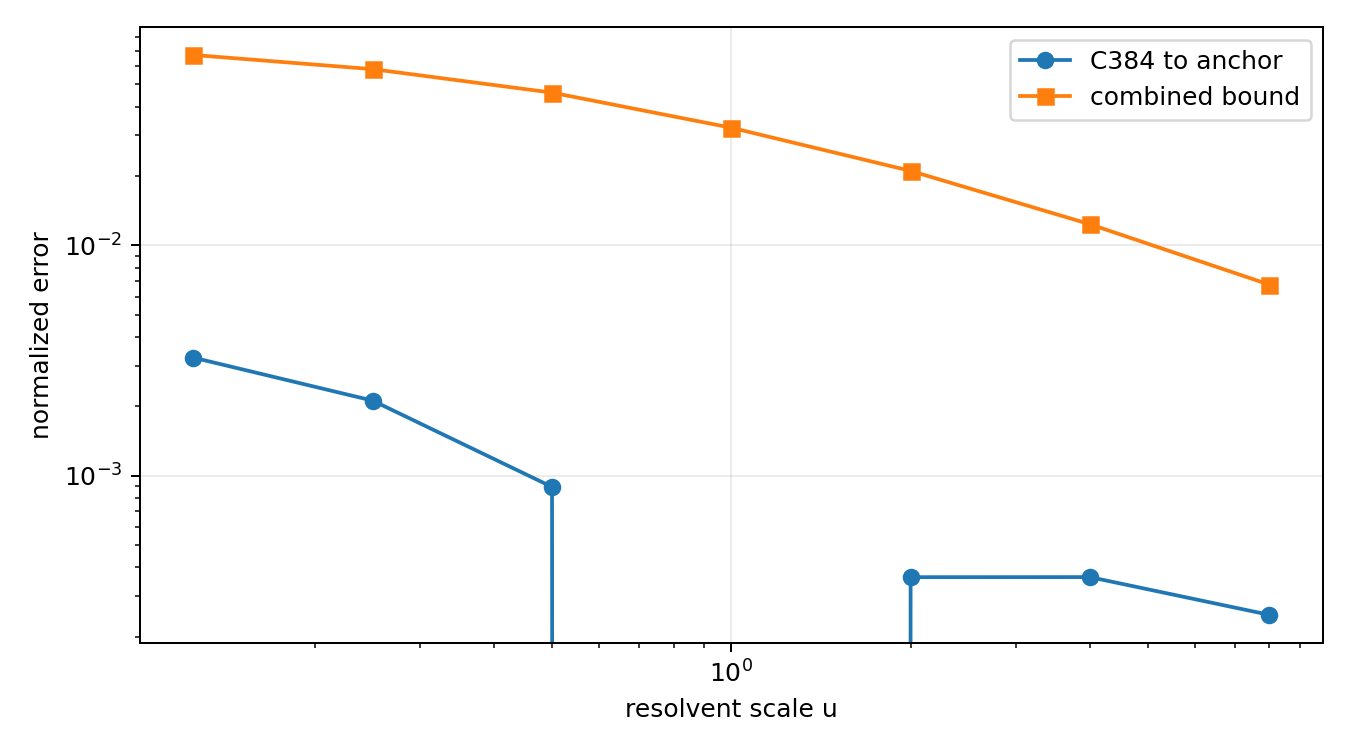
\includegraphics[width=0.78\textwidth]{FIN_Programs_517_526_Figures/p523_C384_bound.png}
\caption{Finite multilevel discrepancy and the transferred $C_{384}$ limit bound.}
\end{figure}

\section{P524 --- portable exact replay of the PSD phase diagram}

All 573 terminal boxes of O218 are exported with hexadecimal endpoints and eleven eigenvalue intervals. The dependency-minimal checker verifies the dyadic rational inequalities without NumPy, SciPy, SymPy or mpmath:
\begin{itemize}
\item 388 boxes have at least one strictly negative eigenvalue upper bound;
\item 182 boxes have all eleven strictly positive lower bounds;
\item three adjacent unresolved boxes merge into the single component
\[
 [0.7008185567101464,\ 0.7008185570593923];
\]
\item the boxes partition $[0,1]$ exactly.
\end{itemize}
Again the replay checks the exported ledger exactly; it does not regenerate the transcendental enclosures.

\section{P525 --- a detector-level admissible error polytope}

For every model pair the nominal total-variation separation $D_{ij}$ yields the conservative half-space
\[
 D_{ij}\ell+D_{ij}\delta+L_{ij}\epsilon
 +2e_{\rm prep}+2e_{\rm POVM}
 +(v_i+v_j)\Delta t+2e_{\rm drift}<D_{ij}.
\]
The seven coordinates are loss fraction $\ell$, dark-count mixture $\delta$, nearest-neighbour coarse graining $\epsilon$, preparation trace distance, POVM variation distance, timing error and configuration drift. The six model pairs produce a nonempty polytope.

A purely hypothetical point
\[
 (0.10,0.01,0.02,0.005,0.005,0.002,0.005)
\]
has worst-case remaining TV margin $0.161408$. The tightest one-coordinate intercept is the timing coordinate, $0.0367286$ in the model's dimensionless time.

\textbf{Physical boundary.} These are algebraic budget variables, not detector specifications, calibrations, raw events or evidence that a laboratory realizes the FIN channel.

\begin{figure}[H]
\centering
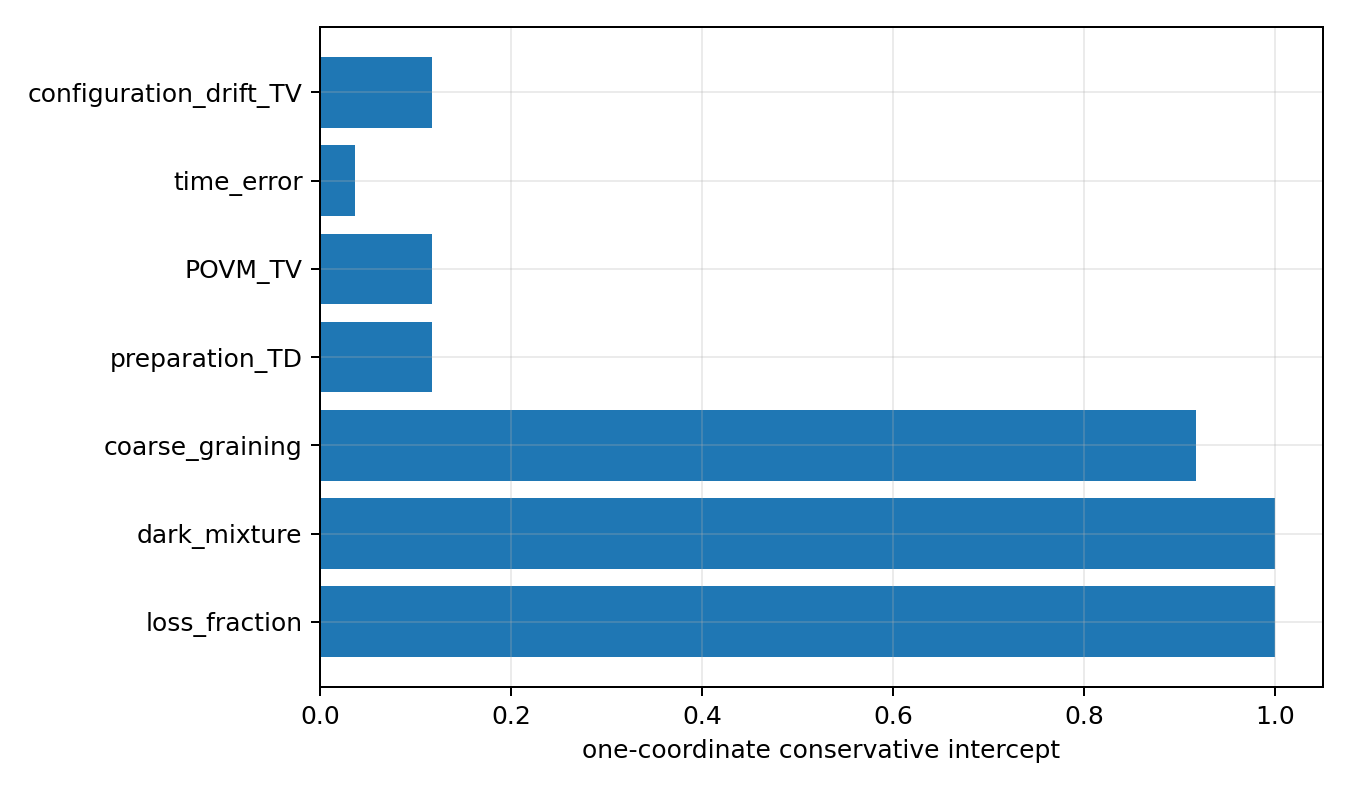
\includegraphics[width=0.78\textwidth]{FIN_Programs_517_526_Figures/p525_detector_polytope_intercepts.png}
\caption{Conservative one-coordinate intercepts of the seven-dimensional error polytope.}
\end{figure}

\section{P526 --- frozen hold-out does not identify a causal law}

A synthetic degree-two parameter-velocity law generated frozen training records at $t=0.2,0.4,0.6,0.8$ and frozen hold-out records at six interlaced times. Polynomial velocity classes of degree zero through three were fitted. The selected degree changes with ridge penalty:
\[
 3,\ 2,\ 3,\ 2
\]
for penalties $0,10^{-6},10^{-4},10^{-2}$. Thus even inside this tiny candidate family, selection depends on the regularization prior.

\begin{theorem}[Finite-record law no-free-lunch]
Let $T$ be the finite union of training and hold-out times and
\[
 b(t)=\prod_{\tau\in T}(t-\tau).
\]
For every smooth fitted path $p(t)$, vector $v$ and scalar $c$, the path $p(t)+cb(t)v$ has identical records at every $t\in T$ and arbitrary off-record behaviour as $c$ varies. Therefore frozen hold-out data can rank a declared finite model family but cannot identify an unrestricted causal bridge law.
\end{theorem}

No strict endpoint was inserted in this experiment; it is not a hidden legacy-to-strict derivation.

\begin{figure}[H]
\centering
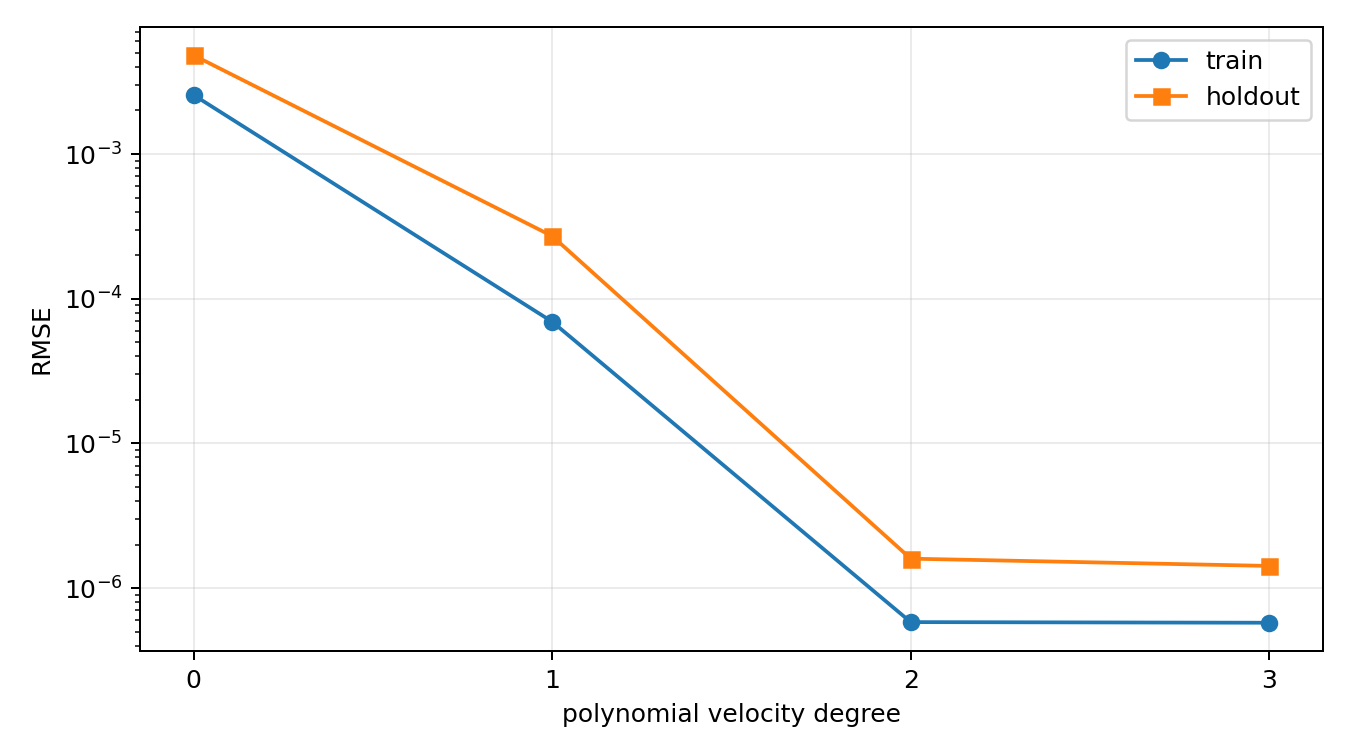
\includegraphics[width=0.78\textwidth]{FIN_Programs_517_526_Figures/p526_holdout_law_selection.png}
\caption{Training and frozen hold-out errors for the unregularized candidate classes.}
\end{figure}

\section{Integrated interpretation}

\subsection{What is now theorem-level}
\begin{enumerate}
\item Generic information-function language does not remove the fourth-jet sign and strength freedom.
\item The supplied focusing DNLS has one connected certified site-centred branch and a certified favourable stability-sign sector near $\omega=1$.
\item The VK transition is unique in $[0.70,0.75]$ and lies in the reported width-$4\times10^{-8}$ interval.
\item The six distinct positive strict frequencies are algebraically linearly independent.
\item Absolute scale is impossible to recover from dimensionless spectral orbits because of the positive rescaling action.
\item The exported Krawczyk and PSD ledgers possess dependency-minimal exact rational replays.
\item Finite records cannot identify an unrestricted parameter-evolution law.
\end{enumerate}

\subsection{What has been falsified or kept conditional}
\begin{itemize}
\item The first explicit temporal Stieltjes hidden-variable completion is unstable despite stationary branch persistence.
\item The scanned phase kicks do not produce a coherently translating localized state.
\item The $C_{384}$ context bound depends on a declared FFT rounding model.
\item Detector tolerances and model-selection data are synthetic, not empirical.
\item No information functional audited here derives the focusing coefficient or its dimension.
\end{itemize}

\claimbox{\textbf{Updated deepest local interpretation.} The strict operator is a dimensionless generator with unusually strong finite spectral arithmetic and a certified capacity to support localization once an attractive fourth-order response is supplied. The new obstruction is not the existence of localized mathematics; it is the origin, sign, scale and operational meaning of the nonlinear response.}

\section{Recommended next bounded studies P527--P536}

\begin{longtable}{@{}p{0.09\textwidth}p{0.25\textwidth}p{0.43\textwidth}p{0.09\textwidth}@{}}
\caption{Next analytical and local-compute programmes.}\\
\toprule
Program & Objective & Acceptance criterion & Priority\\
\midrule
\endfirsthead
\toprule
Program & Objective & Acceptance criterion & Priority\\
\midrule
\endhead
P527 & Axiomatic fourth-jet representation theorem & State minimal information axioms and prove whether they force a unique quartic sign; otherwise classify the complete coefficient cone. & 10/10\\
P528 & Independent O223 exact replay & Export rational state, inertia and implicit-derivative ledgers and reproduce the 208+207 certificates dependency-minimally. & 9/10\\
P529 & Validated nonlinear orbital dynamics & Use a validated integrator and modulation coordinates to test perturbations on both sides of $\omega_*$. & 10/10\\
P530 & Passive memory-realization classification & Search positive-real, Hamiltonian and metriplectic hidden completions; prove a stable class or a realization-level obstruction. & 10/10\\
P531 & Long-time moving-breather audit & Replace finite kick scans by continuation in velocity and a radiation/resonance obstruction test. & 8/10\\
P532 & Quantitative six-torus recurrence & Derive Diophantine recurrence bounds and equidistribution diagnostics while keeping absolute time explicitly unsourced. & 8/10\\
P533 & Exact interval radix-two $C_{384}$ checker & Remove the FFT-model premise from P523 using outward interval twiddle factors and response normalization. & 9/10\\
P534 & Independent transcendental PSD generator & Recompute P514 signs with rational Taylor/argument-reduction bounds rather than replaying mpmath output. & 8/10\\
P535 & Detector-specification inverse map & Convert the P525 half-spaces into platform-neutral minimum component specifications and a raw-event schema, still conditional on apparatus. & 9/10\\
P536 & Law-complexity and prior theorem & Compare MDL, Sobolev, analytic and causal priors and prove which conclusions are invariant under prior class. & 9/10\\
\bottomrule
\end{longtable}

P527 is the conceptual priority because it targets the precisely typed missing fourth-order object. P530 is the most important falsification programme after P521. P529 is the strongest direct upgrade of the certified stability signs to nonlinear evolution.

\section{Reproducibility}

Primary artifacts:
\begin{itemize}
\item \path{fin_programs_517_526_research.py};
\item \path{fin_p518_p524_stdlib_checker.py};
\item \path{test_fin_programs_517_526.py};
\item \path{FIN_Programs_517_526_Results.json};
\item \path{FIN_Programs_517_526_Summary.csv};
\item \path{FIN_P518_Krawczyk_Replay_Certificate.json};
\item \path{FIN_P524_PSD_Replay_Certificate.json};
\item \path{FIN_Programs_517_526_Figures/}.
\end{itemize}

Replay commands:
\begin{verbatim}
MPLCONFIGDIR=/tmp/fin-mpl-1052 \
  python3 fin_programs_517_526_research.py
python3 fin_p518_p524_stdlib_checker.py
MPLCONFIGDIR=/tmp/fin-mpl-1052 \
  python3 -m unittest -v test_fin_programs_517_526.py
pdflatex -interaction=nonstopmode -halt-on-error \
  FIN_Programs_517_526_Fourth_Jet_Stability_and_Clock_Report_EN.tex
\end{verbatim}

The batch uses matrices of order at most 96, 801 replayed Krawczyk inequalities, 208 frequency charts, 207 interface boxes, 573 replayed PSD boxes, 15 finite DNLS trajectories and finite synthetic probability tables. It is designed for an ordinary local workstation.

\section{Final verdict and nonclaims}

P517--P526 materially strengthen the finite mathematical FIN programme. The localized branch and its favourable stability-sign sector are no longer floating numerical observations. The frequency arithmetic expands from one irrational ratio to a maximal six-frequency independence theorem. The context and PSD certificates gain portable replay layers. The detector and law studies acquire explicit admissible and impossible regions.

The same batch closes several tempting shortcuts. Generic Shannon/Fisher/compression language does not generate the attractive fourth-order response. Stationary memory robustness does not imply temporal memory stability. A large circular displacement after a phase kick does not imply transport of a localized object. A six-frequency quasiperiodic clock does not generate an absolute second. Frozen hold-out does not identify an unrestricted causal bridge law.

No result here discharges QW-2191, selects canonical orientation, creates physical units, sources the focusing law from FIN, completes the Legacy*--strict bridge, transfers a legacy physical role, supplies laboratory evidence, derives particles, Standard Model, gravity or $L_{\rm total}$, or closes a Theory of Everything.

\end{document}
